%%%%%%%%%%%%%%%%%%%%%%%%%%%%%%%%%%%%%%%%%%%%%%%%%%%%%%%%%%%%%%%%%%%%%%%%%%%%%
%
%  System        : 
%  Module        : 
%  Object Name   : $RCSfile$
%  Revision      : $Revision$
%  Date          : $Date$
%  Author        : $Author$
%  Created By    : Robert Heller
%  Created       : Mon Nov 25 10:02:10 2019
%  Last Modified : <220902.0854>
%
%  Description 
%
%  Notes
%
%  History
% 
%%%%%%%%%%%%%%%%%%%%%%%%%%%%%%%%%%%%%%%%%%%%%%%%%%%%%%%%%%%%%%%%%%%%%%%%%%%%%
%
%    Copyright (C) 2019  Robert Heller D/B/A Deepwoods Software
%			51 Locke Hill Road
%			Wendell, MA 01379-9728
%
%    This program is free software; you can redistribute it and/or modify
%    it under the terms of the GNU General Public License as published by
%    the Free Software Foundation; either version 2 of the License, or
%    (at your option) any later version.
%
%    This program is distributed in the hope that it will be useful,
%    but WITHOUT ANY WARRANTY; without even the implied warranty of
%    MERCHANTABILITY or FITNESS FOR A PARTICULAR PURPOSE.  See the
%    GNU General Public License for more details.
%
%    You should have received a copy of the GNU General Public License
%    along with this program; if not, write to the Free Software
%    Foundation, Inc., 675 Mass Ave, Cambridge, MA 02139, USA.
%
% 
%
%%%%%%%%%%%%%%%%%%%%%%%%%%%%%%%%%%%%%%%%%%%%%%%%%%%%%%%%%%%%%%%%%%%%%%%%%%%%%

\chapter{ESP32QuadSMCSense: Quad Motor Control and Sense base board for an ESP32 Dev Kit MCU board}

This is a circuit board that supports an ESP32 Dev Kit board or TTGO-T1 board
controlling four stall-motor turnout motors for a model railroad. It also has
sense logic to return the state of the turnouts, using one pole of the DPDT
contacts in the stall-motor (typical of Tortoise stall-motors). This circuit
board provides connections to a LCC CAN network via RJ45 connectors, the
ability to inject and extract 12V power from the LCC CAN network, and a 5V
power supply from the LCC CAN network 12V power bus.

\section{GPIO Pins Used.}

This board uses eight GPIO pins:

\begin{description}
\item[GPIO0] Motor Select 1: select the position of stall motor 
1. 
\item[GPIO12] Motor Select 2: select the position of stall motor 
2. 
\item[GPIO34] Point Sense 1: return the state of the points for 
stall motor 1. 
\item[GPIO35] Point Sense 2: return the state of the points for 
stall motor 2. 
\item[GPIO15] Motor Select 3: select the position of stall motor 
3. 
\item[GPIO25] Motor Select 4: select the position of stall motor 
4. 
\item[GPIO32] Point Sense 3: return the state of the points for 
stall motor 3. 
\item[GPIO33] Point Sense 4: return the state of the points for 
stall motor 4. 
\end{description}

Each of the motor drive circuits is through a TC4428, which can drive up to
1.5A, which is way more needed to drive typical stall motor. It is enough to
drive a pair of stall motors, wired in parallel as would be the case for a
cross over. 

\section{Circuit Description}

\begin{figure}[hbpt]\begin{centering}%
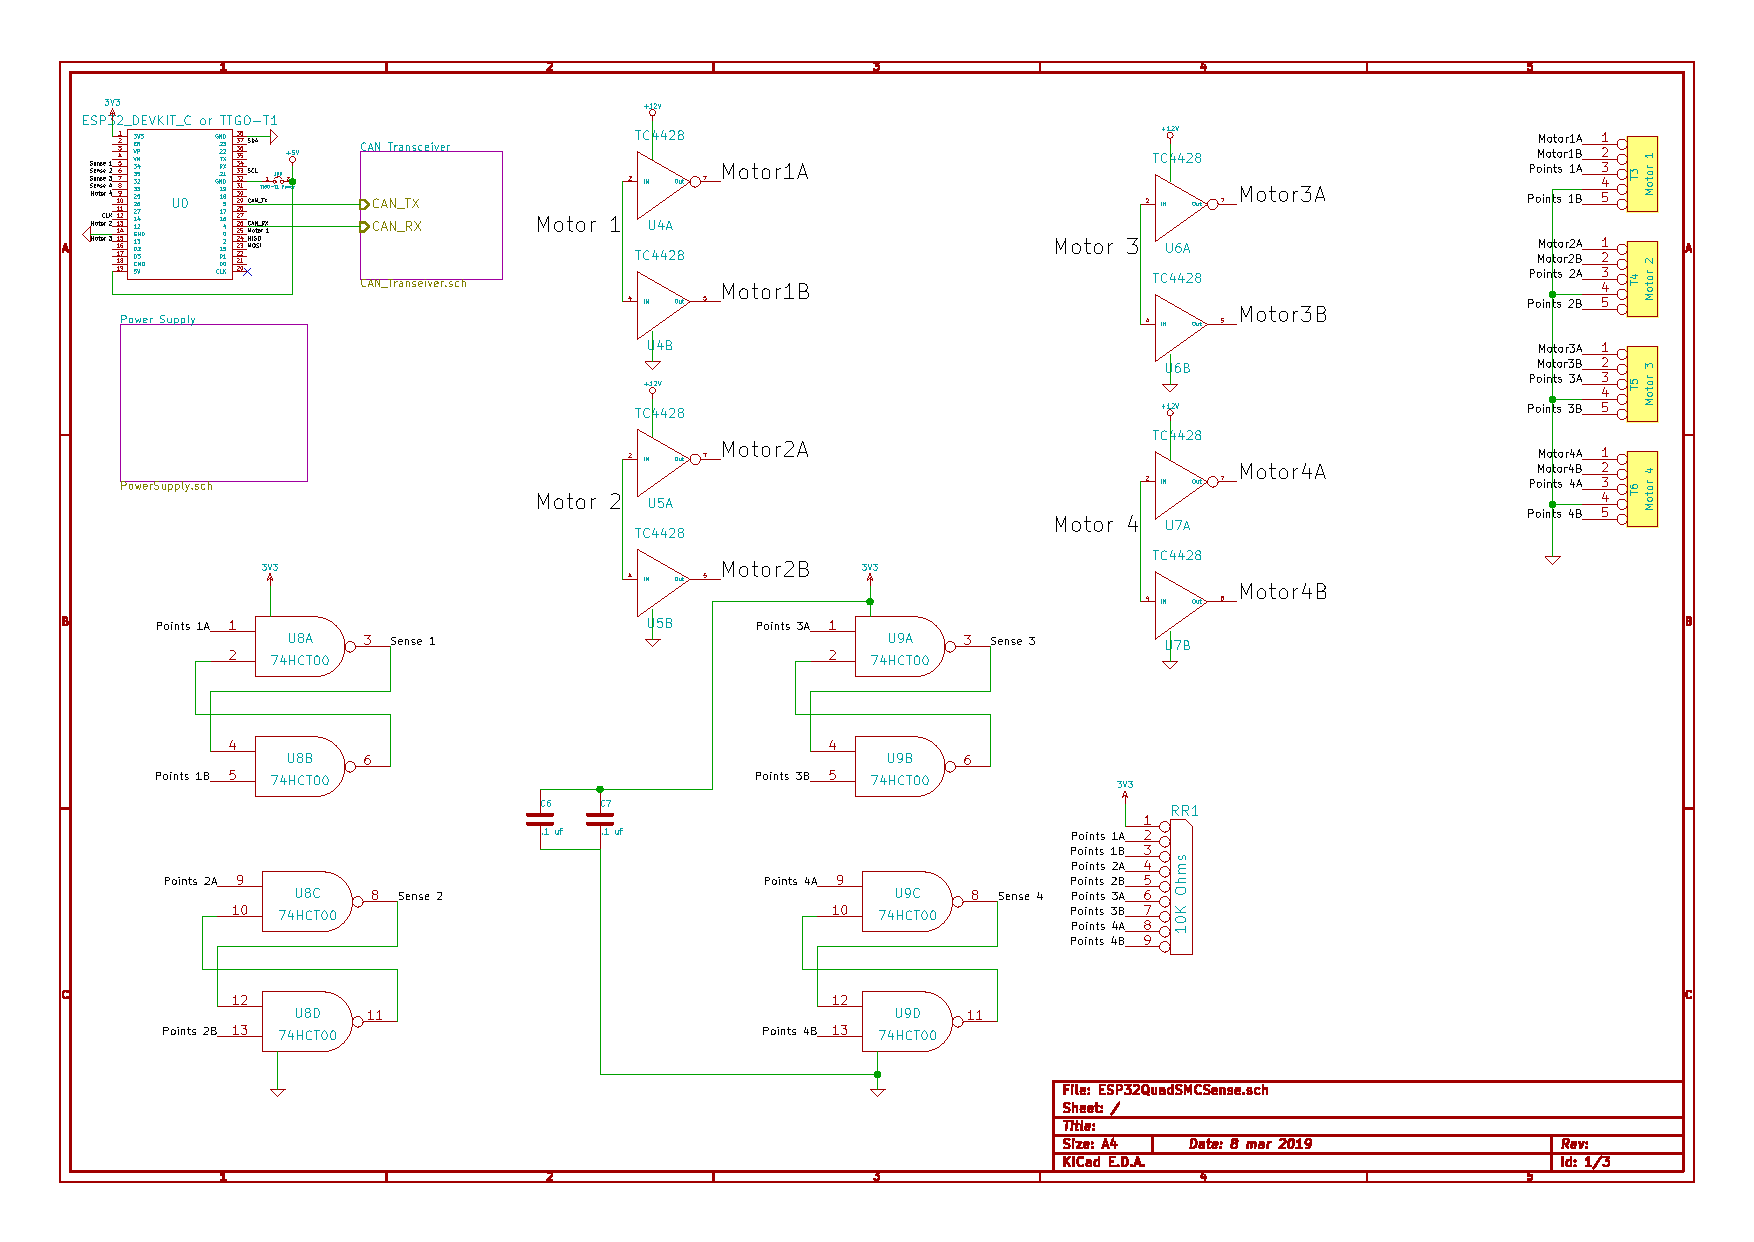
\includegraphics[width=5in]{ESP32QuadSMCSense-1.pdf}
\caption{Circuit Diagram of the ESP32QuadSMCSense, page 1 (ESP32 MCU and Driver and Sense)}
\end{centering}\end{figure}
\begin{figure}[hbpt]\begin{centering}%
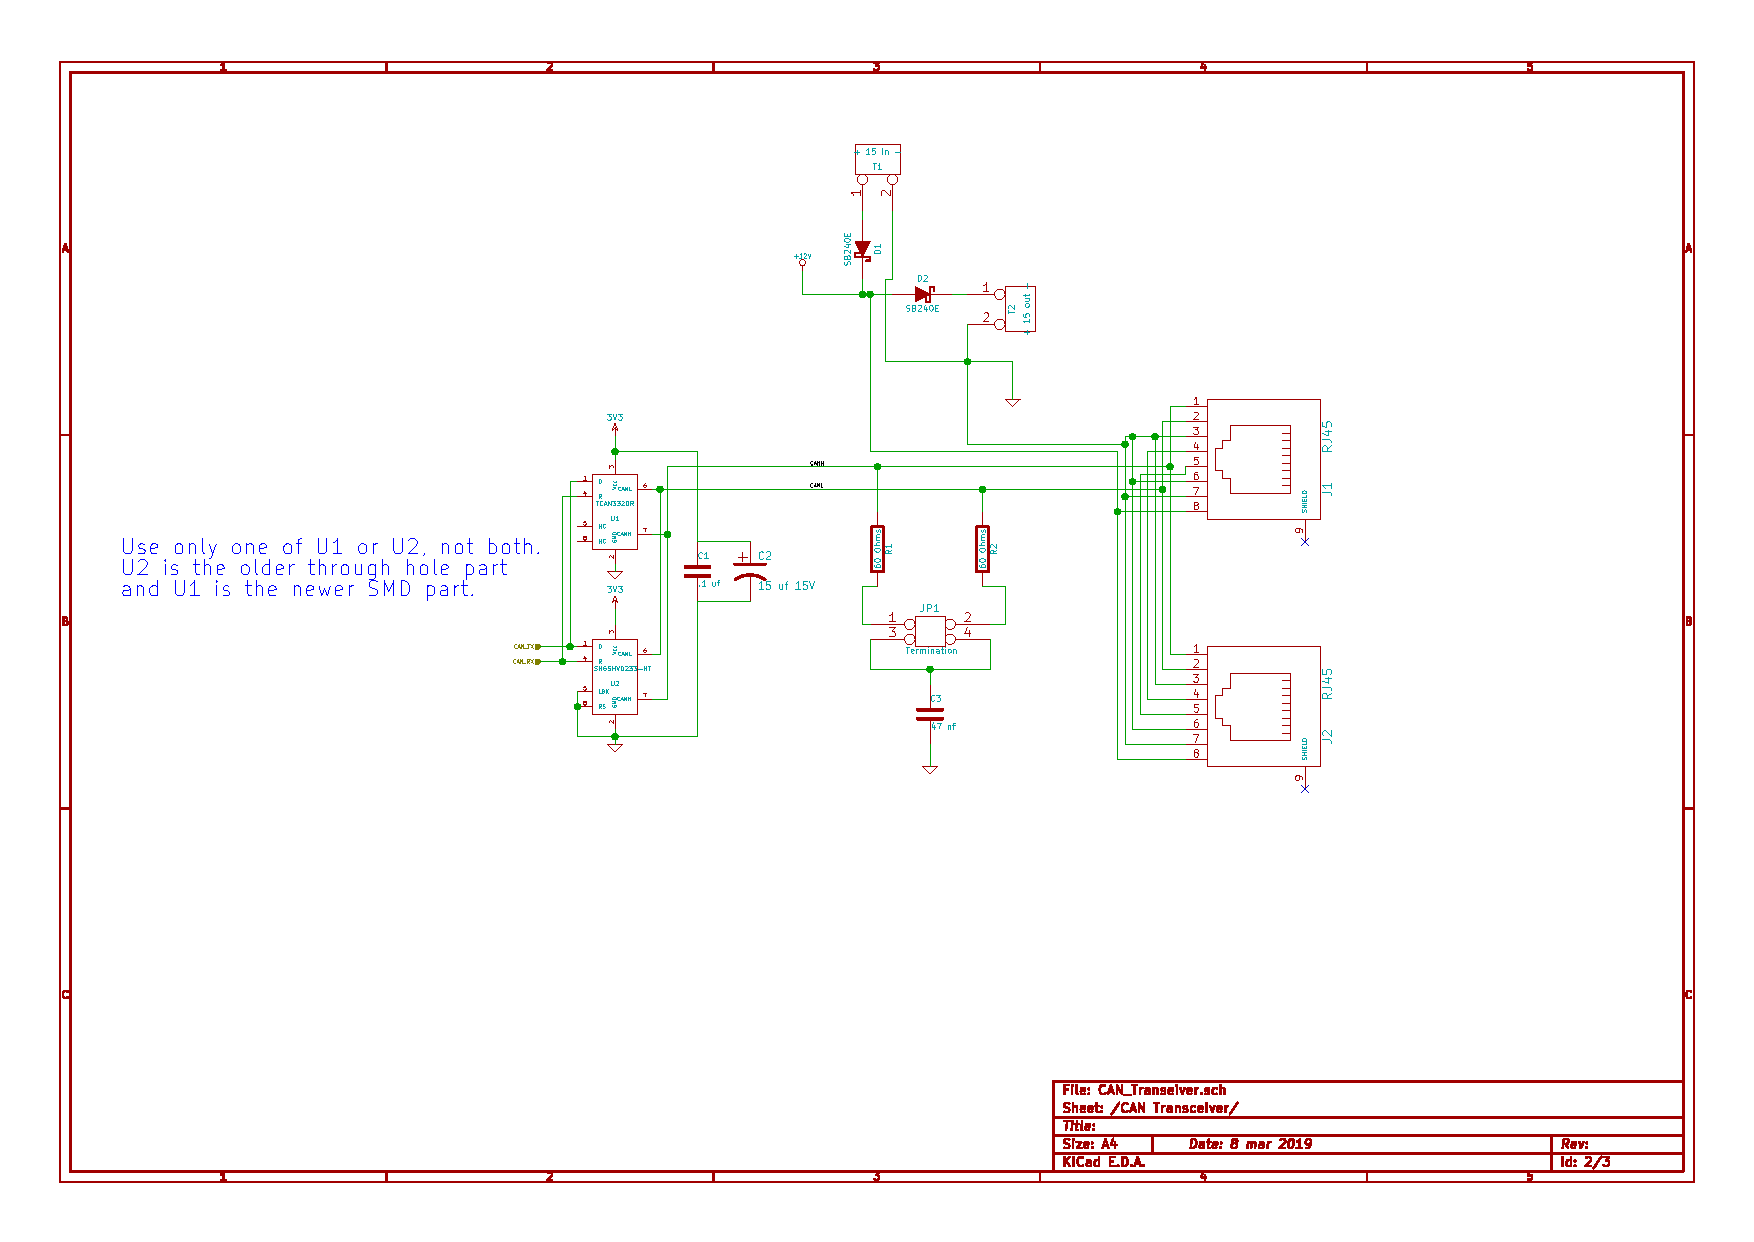
\includegraphics[width=5in]{ESP32QuadSMCSense-2.pdf}
\caption{Circuit Diagram of the ESP32QuadSMCSense, page 2 (CAN Transceiver)}
\end{centering}\end{figure}
\begin{figure}[hbpt]\begin{centering}%
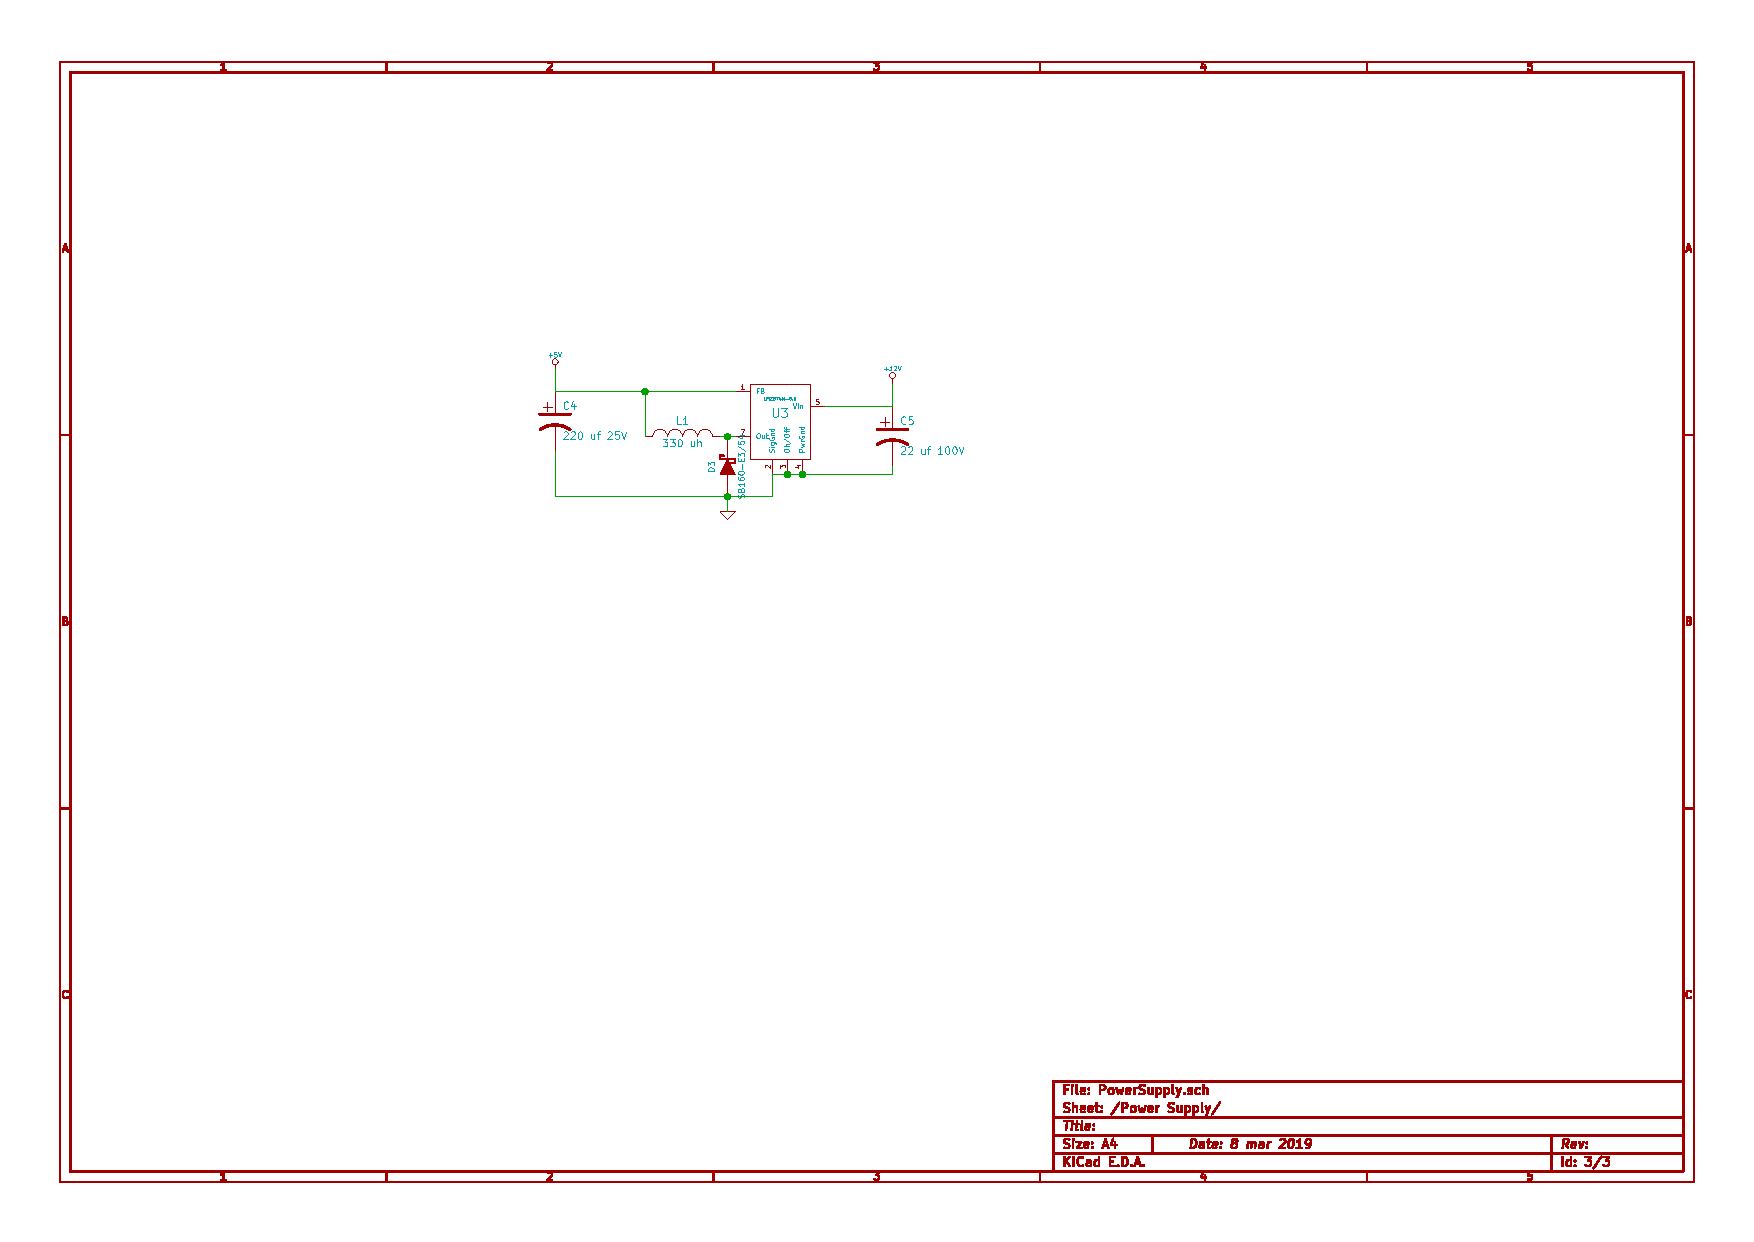
\includegraphics[width=5in]{ESP32QuadSMCSense-3.pdf}
\caption{Circuit Diagram of the ESP32QuadSMCSense, page 3 (Power Supply)}
\end{centering}\end{figure}
This circuit contains two sections.  There is an output section that contains 
four TC4428 chips.  Each chip has a non-inverting and an inverting driver. The 
inputs of both drivers are connected to one of the motor GPIO pins.  The 
output are wired to the terminal block for a one of the motors. For any given 
logic state of the motor control output, one of the drivers is ``on'' and the 
other is ``off'', thus one motor terminal is ground and one is raised to the 
12V supply.  This means alternative states of the logic line will drive the 
stall motor in alternative directions.

The other section is a quartet of flip-flop debounce circuits, one for each
of two SPDT switch contacts that report the position of the turnout points.
The output of these flip-flops goes to a quartet of GPIO input pins.

Also on the board is a CAN Transceiver and power supply for the Pocket Beagle.

\section{Parts List}

\begin{table}[htp]
\begin{centering}\begin{tabular}{|l|l|p{1in}|l|p{.5in}|}
\hline
Value&Quantity&References&Mouser Part Number \\
\hline
.1 uf&2&C1 C2&581-SR201C104KARTR1 \\
\hline
10 uf 35V&1&C3&667-ECA-1HM100I \\
\hline
RPi\_GPIO&1&J0&855-M20-6102045 \\
\hline
10K Ohms&1&RR1&652-4609X-1LF-10K \\
\hline
Motor 1;Motor 2;Motor 3;Motor 4&4&T1 T2 T3 T4&651-1725685 \\
\hline
+ 12V -&1&T5&651-1725656 \\
\hline
TC4428&4&U1 U2 U3 U4&579-TC4428VPA \\
\hline
74HCT00&2&U5 U6&595-SN74AHC00N \\
\hline
.1 uf&1&C1&21RZ310-RC\\
\hline
15 uf 63V&1&C2&710-860080773002\\
\hline
47 nf&1&C3&75-1C10Z5U473M050B\\
\hline
SB240E&2&D1 D2&625-SB240-E3\\
\hline
RJ45&2&J1 J2&710-615008144221\\
\hline
Termination&1&JP1&649-67997-404HLF\\
\hline
60 Ohms&2&R1 R2&71-RN60C60R0B/R\\
\hline
+ 15 in -;+ 15 out -&2&T1 T2&651-1725656\\
\hline
TCAN332DR&1&U1&595-TCAN332DR\\
\hline
SN65HVD233-HT&1&U2&595-SN65HVD233SJD\\
\hline
220 uf 25V&1&C4&140-REA221M1EBK0811P\\
\hline
22 uf 100V&1&C5&140-REA220M2ABK0811P\\
\hline
SB160-E3/54&1&D3&625-SB160-E3\\
\hline
330 uh&1&L1&PE-52627NL\\
\hline
LM2574N-5.0&1&U3&926-LM2574N-5.0/NOPB\\
\hline
\end{tabular}
\caption{Parts list for ESP32QuadSMCSense board.}
\end{centering}\end{table}\footnote{Mouser Project link: 
\url{http://www.mouser.com/ProjectManager/ProjectDetail.aspx?AccessID=330542c522},
\url{http://www.mouser.com/ProjectManager/ProjectDetail.aspx?AccessID=82b1e6b259}, and
\url{http://www.mouser.com/ProjectManager/ProjectDetail.aspx?AccessID=ae58a2d985}.}


The only parts that might be substituted are T1 though T4 (the Motor
terminals) and T5 (the 12 to 16 Volts terminals). The parts listed are for
screw terminals for the Motor terminals and the motor power terminals. Feel
free to select either pin arrays or spring terminals for the T1, T2, T3, T4
and T5. You only need one CAN transciever. One of the parts is a through hole
version (which is much more expensive) and the other is SMD. The SMD part can
be hand soldered. The board supports using either a pair a 18-pin headers for
a TTGO-T1 MCU board or a pair a 19-pin headers for a ESP32 Dev Kit Board.

\section{Circuit Board Layout}

\begin{figure}[hbpt]\begin{centering}%
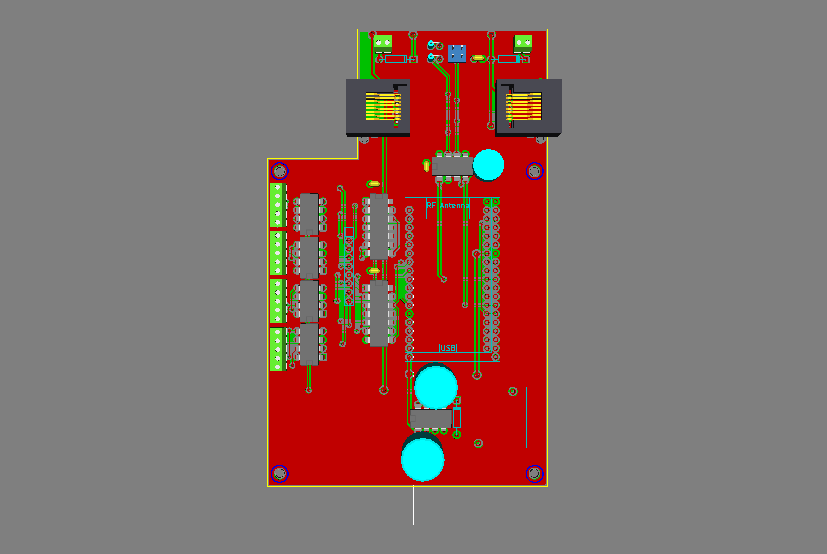
\includegraphics[width=5in]{ESP32QuadSMCSense3DTop.png}
\caption{3D rendering of the ESP32QuadSMCSense board}
\end{centering}\end{figure}
\begin{figure}[hbpt]\begin{centering}%
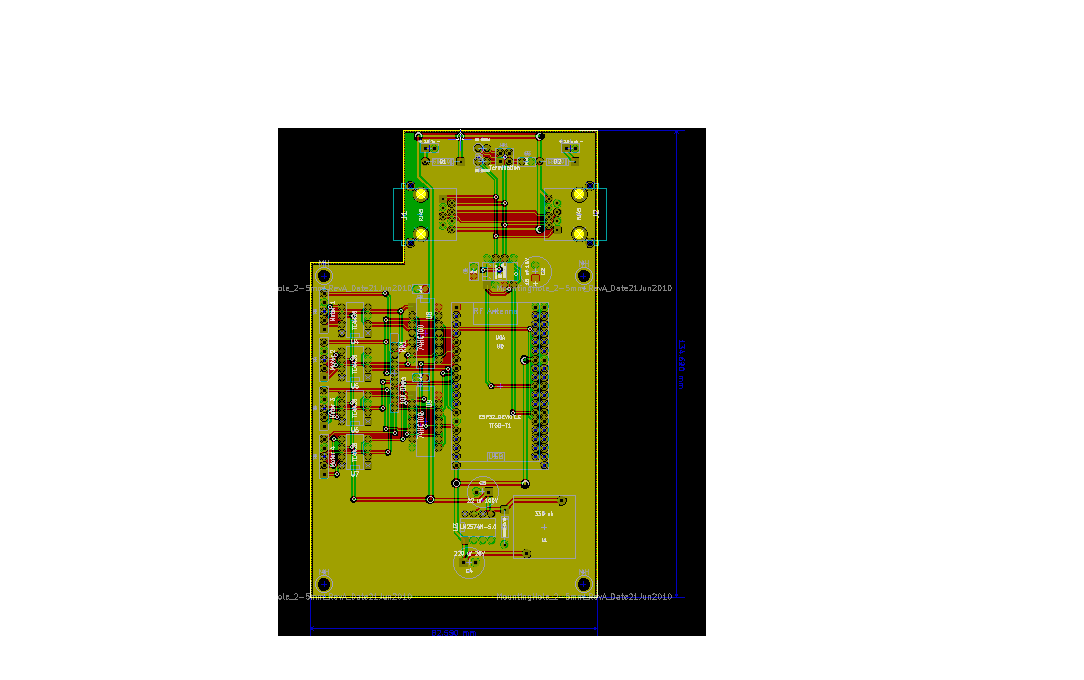
\includegraphics[width=5in]{ESP32QuadSMCSense.png}
\caption{Fabrication image of the ESP32QuadSMCSense board}
\end{centering}\end{figure}
Board assembly is straight forward. You need to be careful orienting the ICs
and the electrolytic capacitor.

Bare circuit boards can be ordered from PCBWay here: 
\url{https://www.pcbway.com/project/shareproject/ESP32QuadSMCSense.html}.

\section{Downloadables and Software Support}

Full design information is available on GitHub here:
\url{https://github.com/RobertPHeller/RPi-RRCircuits/tree/master/ESP32QuadSMCSense}.

An OpenMRN Lite program that supports this board is available here:
\url{https://github.com/RobertPHeller/RPi-RRCircuits/tree/master/ESP32MRNSketches/ESP32QuadSMCSense}.



